\documentclass{asaproc}

\usepackage{graphics}

%\usepackage{times}
%If you have times installed on your system, please
%uncomment the line above

%For figures and tables to stretch across two columns
%use \begin{figure*} \end{figure*} and
%\begin{table*}\end{table*}
% please place figures & tables as close as possible
% to text references


\newcommand{\be}{\begin{equation}}
\newcommand{\ee}{\end{equation}}

 \title{Sample Title---Center in 12-Point Bold}

%input all authors' names

\author{Author Name$^1$, Author Name$^2$, Author Name$^1$\\
First Author Affiliation$^1$\\
Second Author Affiliation$^2$}

%input affiliations

%{USDA Forest Service Forest Products Laboratory}

\begin{document}

\maketitle


\begin{abstract}
This is sample text in 10-point Times New Roman type and needs to be completely replaced before submitting your paper. This is sample text and needs to be completely replaced before submitting your paper. This is sample text and needs to be completely replaced before submitting your paper. This is sample text and needs to be completely replaced before submitting your paper. This is sample text and needs to be completely replaced before submitting your paper. This is sample text and needs to be completely replaced before submitting your paper. This is sample text and needs to be completely replaced before submitting your paper. This is sample text and needs to be completely replaced before submitting your paper. This is sample text and needs to be completely replaced before submitting your paper. This is sample text and needs to be completely replaced before submitting your paper. This is sample text and needs to be completely replaced before submitting your paper.
\begin{keywords}
Please place 3--5 key words here.
\end{keywords}
\end{abstract}


\section{Primary Subhead Centered, Title Case in 10-Point Bold}

This is sample text and needs to be completely replaced before submitting your paper. This is sample text and needs to be completely replaced before submitting your paper. This is sample text and needs to be completely replaced before submitting your paper. This is sample text and needs to be completely replaced before submitting your paper.

This is sample text and needs to be completely replaced before submitting your paper. This is sample text and needs to be completely replaced before submitting your paper.  This is sample text and needs to be completely replaced before submitting your paper. This is sample text and needs to be completely replaced before submitting your paper.

This is sample text and needs to be completely replaced before submitting your paper. This is sample text and needs to be completely replaced before submitting your paper. This is sample text and needs to be completely replaced before submitting your paper. This is sample text in 10-point Times New Roman type and needs to be completely replaced before submitting your paper. This is sample text and needs to be completely replaced before submitting your paper.

\subsection{Secondary Head}

This is sample text and needs to be completely replaced before submitting your paper. This is sample text and needs to be completely replaced before submitting your paper. This is sample text and needs to be completely replaced before submitting your paper. This is sample text and needs to be completely replaced before submitting your paper.

This is sample text and needs to be completely replaced before submitting your paper. This is sample text and needs to be completely replaced before submitting your paper.  This is sample text and needs to be completely replaced before submitting your paper. This is sample text and needs to be completely replaced before submitting your paper.

This is sample text and needs to be completely replaced before submitting your paper. This is sample text and needs to be completely replaced before submitting your paper. This is sample text and needs to be completely replaced before submitting your paper. This is sample text in 10-point Times New Roman type and needs to be completely replaced before submitting your paper. This is sample text and needs to be completely replaced before submitting your paper.

This is sample text and needs to be completely replaced before submitting your paper. This is sample text and needs to be completely replaced before submitting your paper. This is sample text and needs to be completely replaced before submitting your paper. This is sample text and needs to be completely replaced before submitting your paper.

This is sample text and needs to be completely replaced before submitting your paper. This is sample text and needs to be completely replaced before submitting your paper.  This is sample text and needs to be completely replaced before submitting your paper. This is sample text and needs to be completely replaced before submitting your paper.

This is sample text and needs to be completely replaced before submitting your paper. This is sample text and needs to be completely replaced before submitting your paper. This is sample text and needs to be completely replaced before submitting your paper. This is sample text in 10-point Times New Roman type and needs to be completely replaced before submitting your paper. This is sample text and needs to be completely replaced before submitting your paper.

\begin{table*}
\caption{\enspace Possible Rankings of $A$, $B$, and $C$ and Corresponding 
Posterior Probabilities.  Because of rounding, not all columns sum to 
one.}\label{tab1}
\begin{tabular*}{\hsize}{@{\extracolsep{\fill}}ccccccc}
\\[-5pt]
                 & 
\multicolumn{1}{c}{\it Errors} & 
\multicolumn{1}{c}{\it Posterior probability} & 
\multicolumn{4}{c}{\it Posterior probability for specified $\beta$}\\
\cline{4-7}
\\[-7pt]
\multicolumn{1}{c}{\it $(R_A,R_B,R_C)$}  & 
\multicolumn{1}{c}{\it $g({\bf R})$} & 
\multicolumn{1}{c}{\it as a function of $\beta$} & 
\multicolumn{1}{c}{\it $\beta =$ .5} & 
\multicolumn{1}{c}{\it $\beta =$ .3} & 
\multicolumn{1}{c}{\it $\beta =$ .1} & 
\multicolumn{1}{c}{\it $\beta =$ .01}\\
\hline
\\[-5pt]
(1, 2, 3)& $0$ & $1 / (1 + 2\beta + 2\beta^{\,2} + \beta^{\,3})$ & 
        .381 & .553 & .819 & .980 \\ 
(1, 3, 2)& $1$ & $\beta/ (1 + 2\beta + 2\beta^{\,2} + \beta^{\,3})$ & 
        .190 & .166 & .082 & .010 \\
(2, 1, 3)& $1$ & $\beta/ (1 + 2\beta + 2\beta^{\,2} + \beta^{\,3})$ & 
        .190 & .166 & .082 & .010 \\
(2, 3, 1)& $2$ & $\beta^{\,2}/ (1 + 2\beta + 2\beta^{\,2} + \beta^{\,3})$ & 
        .095 & .050 & .008 & .000 \\
(3, 1, 2)& $2$ & $\beta^{\,2}/ (1 + 2\beta + 2\beta^{\,2} + \beta^{\,3})$ &  
         .095 &  .050 &  .008 &  .000 \\
(3, 2, 1)& $3$ & $\beta^{\,3}/ (1 + 2\beta + 2\beta^{\,2} + \beta^{\,3})$ & 
         .048 &  .015 &  .001 &   .000 \\
\hline
\end{tabular*}
\end{table*} 

\subsubsection{This is a tertiary head} 

This is sample text and needs to be completely replaced before submitting your paper. This is sample text and needs to be completely replaced before submitting your paper. This is sample text and needs to be completely replaced before submitting your paper. This is sample text and needs to be completely replaced before submitting your paper.

This is sample text and needs to be completely replaced before submitting your paper. This is sample text and needs to be completely replaced before submitting your paper.  This is sample text and needs to be completely replaced before submitting your paper. This is sample text and needs to be completely replaced before submitting your paper.

This is sample text and needs to be completely replaced before submitting your paper. This is sample text and needs to be completely replaced before submitting your paper. This is sample text and needs to be completely replaced before submitting your paper. This is sample text in 10-point Times New Roman type and needs to be completely replaced before submitting your paper. This is sample text and needs to be completely replaced before submitting your paper.

\section{Another Primary Subhead}

This is sample text and needs to be completely replaced before submitting your paper. This is sample text and needs to be completely replaced before submitting your paper. This is sample text and needs to be completely replaced before submitting your paper. This is sample text and needs to be completely replaced before submitting your paper.

This is sample text and needs to be completely replaced before submitting your paper. This is sample text and needs to be completely replaced before submitting your paper.  This is sample text and needs to be completely replaced before submitting your paper. This is sample text and needs to be completely replaced before submitting your paper.

This is sample text and needs to be completely replaced before submitting your paper. This is sample text and needs to be completely replaced before submitting your paper. This is sample text and needs to be completely replaced before submitting your paper. This is sample text in 10-point Times New Roman type and needs to be completely replaced before submitting your paper. This is sample text and needs to be completely replaced before submitting your paper.\begin{eqnarray}
\hat{\rho} & \equiv & \sum_{j=1}^J
\sum_{i=1}^n (x_{ij} - \bar{x}_{\cdot \cdot})(y_{ij} - \bar{y}_{\cdot
j}) \nonumber \\
& \div & \sqrt{
\sum_{j=1}^J \sum_{i=1}^n (x_{ij} - \bar{x}_{\cdot \cdot})^2
\sum_{j=1}^J \sum_{i=1}^n (y_{ij} - \bar{y}_{\cdot j})^2
}
. \nonumber
\end{eqnarray}
Version 2 uses the maximum likelihood estimate of $\rho$.


This is sample text and needs to be completely replaced before submitting your paper. This is sample text and needs to be completely replaced before submitting your paper. This is sample text and needs to be completely replaced before submitting your paper. This is sample text and needs to be completely replaced before submitting your paper.

This is sample text and needs to be completely replaced before submitting your paper. This is sample text and needs to be completely replaced before submitting your paper.  This is sample text and needs to be completely replaced before submitting your paper. This is sample text and needs to be completely replaced before submitting your paper.

This is sample text and needs to be completely replaced before submitting your paper. This is sample text and needs to be completely replaced before submitting your paper. This is sample text and needs to be completely replaced before submitting your paper. This is sample text in 10-point Times New Roman type and needs to be completely replaced before submitting your paper. This is sample text and needs to be completely replaced before submitting your paper.


\begin{figure*}
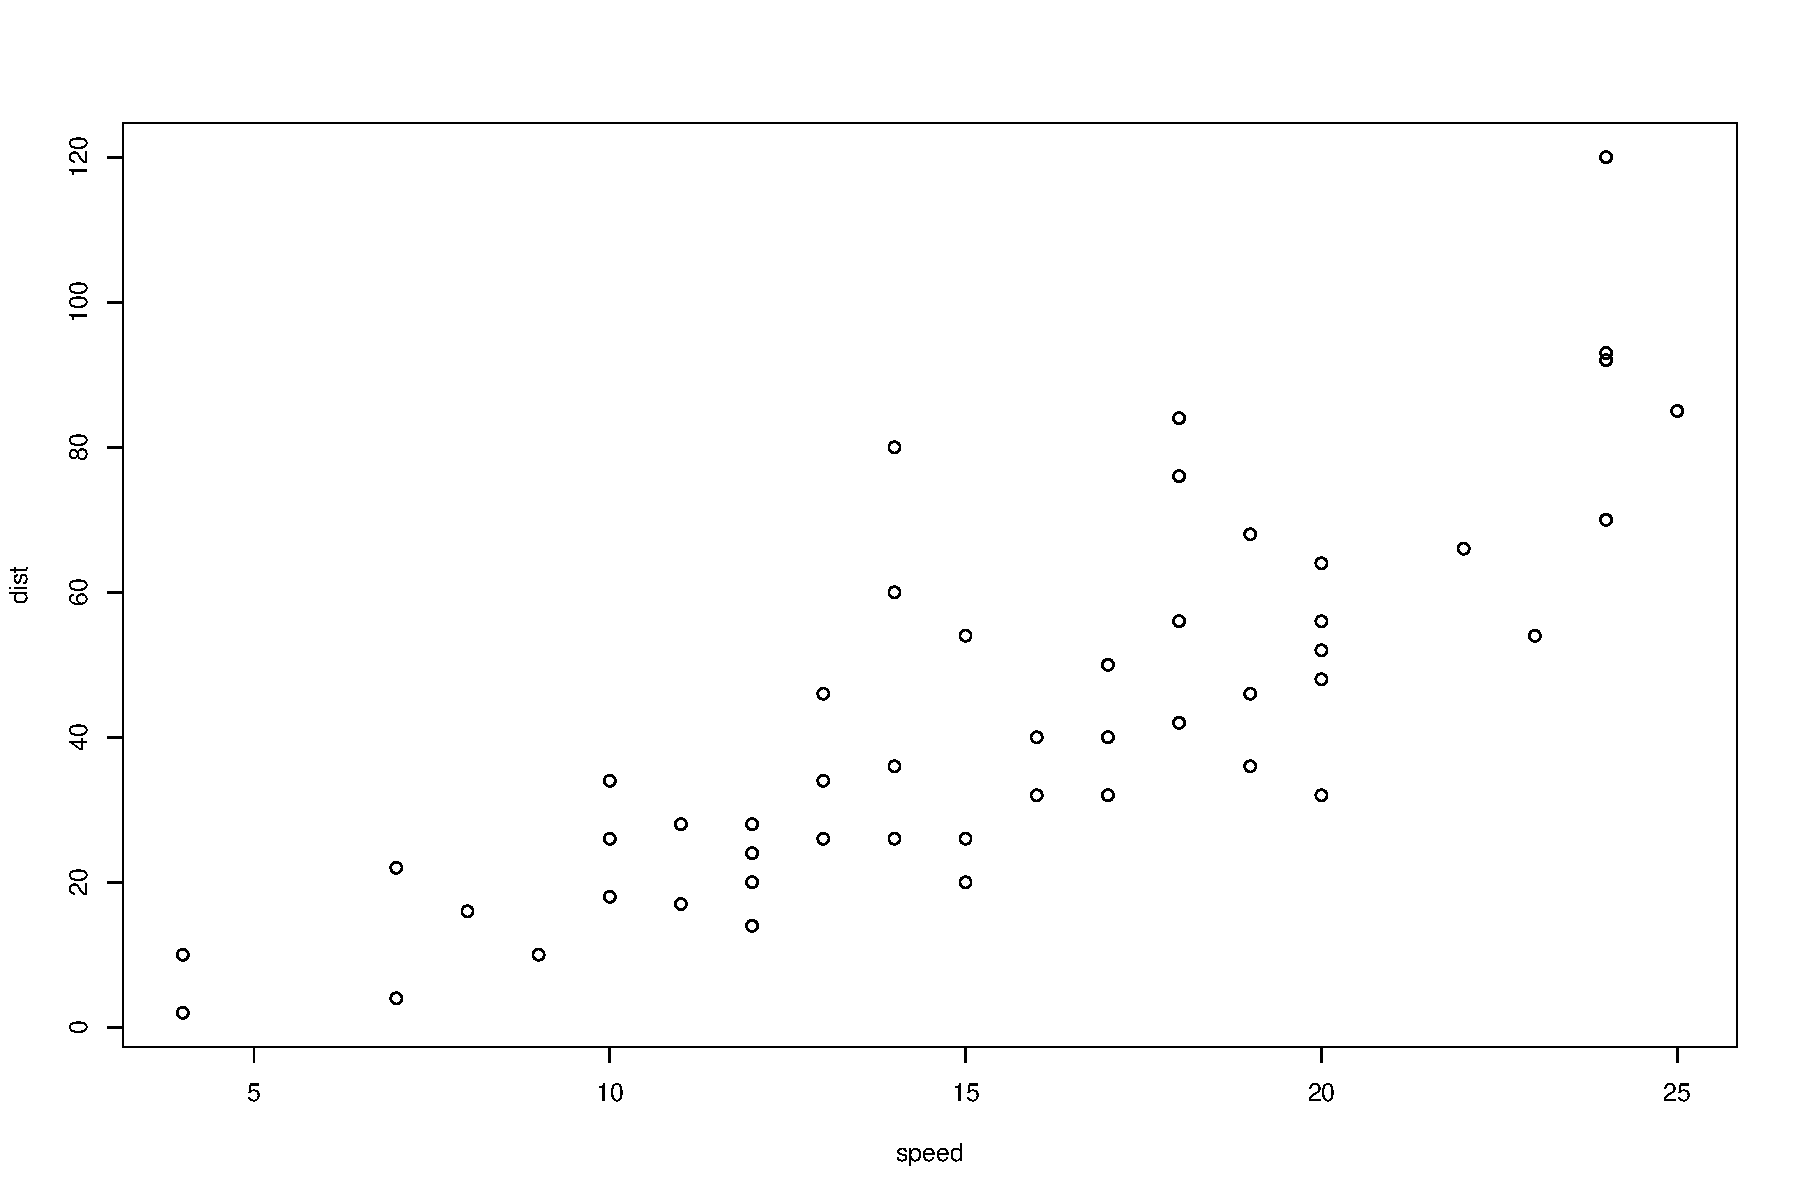
\includegraphics{./Figs/unnamed-chunk-1-1.pdf}
\vspace{12pc}
\caption{Actual confidence interval coverages,
$J = 4$, $\rho = .85$, nominal confidence level = .75,
quantile = .01}
\end{figure*}
However, for large $J$ and small $n$, the version 1 approach does not perform as well.


\begin{table}[b]
\caption{\enspace Possible Rankings of $A$, $B$, and $C$ and Corresponding 
Posterior Probabilities.  Because of rounding, not all columns sum to 
one.}\label{tab2}
\begin{tabular*}{\hsize}{@{\extracolsep{\fill}}cccc}
\\[-5pt]
\multicolumn{1}{c}{\it $\beta =$ .5} & 
\multicolumn{1}{c}{\it $\beta =$ .3} & 
\multicolumn{1}{c}{\it $\beta =$ .1} & 
\multicolumn{1}{c}{\it $\beta =$ .01}\\
\hline
\\[-5pt]
.381 & .553 & .819 & .980 \\ 
        .190 & .166 & .082 & .010 \\
        .190 & .166 & .082 & .010 \\
        .095 & .050 & .008 & .000 \\
         .095 &  .050 &  .008 &  .000 \\
         .048 &  .015 &  .001 &   .000 \\
\hline
\end{tabular*}
\end{table} 




\begin{references}
{\footnotesize
\itemsep=3pt

\item {\em Annual Book of ASTM Standards, Volume 4.10}, Committee D-7,
American Society for Testing and Materials, West Conshohocken, Pennsylvania.
\item Cochran, W.G. (1957),  ``Analysis of Covariance: Its Nature and Uses,''
{\em Biometrics}, {\bf 13}, 261-281.
\item Cox, D.R. (1957),  ``The Use of a Concomitant Variable in Selecting an
Experimental Design,''  {\em Biometrika}, {\bf 44}, 150-158.
\item David, H.A. and Gunnik, J.L. (1997), ``The Paired {\em t} Test
Under Artificial Pairing,'' {\em The American Statistician}, {\bf 51},
9--12.
\item Gibbons, R.D. (1994), {\em Statistical Methods for Groundwater
Monitoring},
John Wiley and Sons, New York.
\item Guttman, I. (1970), {\em Statistical Tolerance Regions:
Classical and Bayesian}, Hafner Publishing Company, Darien,
Connecticut.
\item Michigan DEQ (1994), {\em Guidance Document, Verification of
Soil Remediation}, Hazardous Waste Program Section, Waste Management
Division, Michigan Department of Environmental Quality, Lansing, Michigan.
\item Owen, D.B. (1963), {\em Factors for one-sided tolerance limits
and for variable sampling plans}, Sandia Corporation Monograph No.
SCR-607 (19th edn).
\item {\em MIL-HDBK-17-1, Composite Materials Handbook, Volume 1,
Guidelines for Characterization of Structural Materials}, Department
of Defense Single Stock Point, Philadelphia, Pennsylvania
(http://www.dodssp.daps.mil).
\item Verrill, S.P. (1993),  ``Predictor Sort Sampling, Tight
{\em T}'s, and the Analysis of Covariance,'' {\em Journal of the American
Statistical Association}, {\bf 88}, 119--124.
\item Verrill, S.P. (1999),  ``When Good Confidence Intervals Go Bad:
Predictor Sort Experiments and ANOVA,'' {\em The American
Statistician}, {\bf 53}, 38--42.
\item Verrill, S.P., Herian, V.L., and Green, D.W. (2002a), ``Predictor
Sort Sampling and Confidence Bounds on Quantiles I: Asymptotic Theory,''
under review.
\item Verrill, S.P., Herian, V.L., and Green, D.W. (2002b), ``Predictor
Sort Sampling and Confidence Bounds on Quantiles II: $k$'s for Small
Samples,'' in preparation.
\item Warren, W.G., and Madsen, B. (1977),  ``Computer-Assisted Experimental Design
in Forest Products Research: A Case Study Based on Testing the 
Duration-of-Load Effect,''  {\em Forest Products Journal}, {\bf 27}, 45-50.

}
\end{references}


\end{document}

